\documentclass{beamer}	
\usecolortheme{wolverine}

\setbeamertemplate{caption}{\raggedright\insertcaption\par}

\usepackage{tabularx}
\usepackage{booktabs}
\usepackage{multirow}
\newcolumntype{C}{>{\centering\arraybackslash}X}
\usepackage{proof}
\usepackage{amsmath}
\usepackage{wasysym}
\usepackage{tikz}
\usetikzlibrary{arrows.meta,positioning,matrix}
\usepackage{tikz-qtree}

\newcommand{\term}[1]{\texttt{#1}}
\newcommand{\li}{\!\multimap\!}
\newcommand{\lotimes}{\!\otimes\!}
\newcommand{\loplus}{\!\oplus\!}
\newcommand{\lin}[1]{\langle#1\rangle}
\newcommand{\lint}[1]{[#1]}
\newcommand{\trans}[1]{\lceil #1 \rceil}
\newcommand{\barkr}[1]{#1^{\leadsto}}
\newcommand{\barkl}[1]{#1^{\rotatebox[origin=c]{180}{$\leadsto$}}}

\title{Syntax-Semantics Interface}
\author{K. Kogkalidis}
\institute{Logic \& Language 2020}

\begin{document}
\date{}
\maketitle

\begin{frame}{Two Key Ideas}
	\small
	\begin{minipage}{0.4\textwidth}
		\centering
		\begin{figure}
			\includegraphics[width=0.5\textwidth]{Frege}
			\caption{Gottlob Frege}
		\end{figure}
	\end{minipage}%
	\begin{minipage}{0.6\textwidth}
		\alert{Principle of Compositionality}\\
		The meaning of a complex expression is derived by its constituent components and their interactions.
	\end{minipage}
	\begin{minipage}{0.6\textwidth}
	\alert{Universal Grammar}\\
	Homomorphism between a syntactic and a semantic algebra associates syntactic operations to semantic operations.
	\end{minipage}%
	\begin{minipage}{0.4\textwidth}
	\centering
		\begin{figure}
			\includegraphics[width=0.5\textwidth]{Montague}
			\caption{Richard Montague}
		\end{figure}
	\end{minipage}

\end{frame}

\begin{frame}{In our case}
	\small
	\begin{tabularx}{0.99\textwidth}{@{}c@{\quad}c@{\quad}c@{\quad}c@{\quad}c@{}}
		\text{syntactic calculus} & $\xrightarrow{\makebox[0.33in]{$h_1$}}$ & \text{semantic calculus} & $\xrightarrow{\makebox[0.33in]{$h_2$}}$ & \text{lexical meaning}\\
				NL / L / .. & & MILL${}_{\li, \lotimes}$ /.. & & IL${}_{\to, \times}$ \\ 
		\\
		\textit{surface form} & & \textit{meaning} & & \textit{meaning} \\
		& &	{\footnotesize(computational)} & & {\footnotesize(lexical)}
	\end{tabularx}
	\vfill	

	For each $h_i$ we will need:
	\begin{itemize}
		\item A map to associate source types to target types 
		\item A map to associate source terms to target terms
	\end{itemize}		
	\begin{flushright}
		remember: $\mathfrak{L}$, $\eta$, $\theta$ of ACGs
	\end{flushright}
\end{frame}

\begin{frame}{Linear Syntax, Intuitionistic Semantics?}
	\small
	\alert{Minimal term syntax for NL}
	\[
	\begin{array}{@{}c@{\quad}c@{}}
	\vcenter{\infer[/ E]{(\Gamma, \Delta) \vdash \term{f} \triangleleft \term{x}: B}{\Gamma \vdash \term{f}: B/A & \Delta \vdash \term{x}: A}} &
	\vcenter{\infer[\backslash E]{(\Gamma, \Delta) \vdash \term{x} \triangleright \term{f}: B}{\Gamma \vdash \term{x}: B & \Delta \vdash \term{f}: A \backslash B}}	\vspace{10pt} \\
	\vcenter{\infer[/ I]{\Gamma \vdash \lambda \term{x} {}^r.\term{f}: B/A}{
		\Gamma, \term{x}: A \vdash \term{f}: B}}
	&
	\vcenter{\infer[\backslash I]{\Gamma \vdash \lambda \term{x} {}^l.\term{f}: A \backslash B}{\term{x}: A, \Gamma \vdash \term{f}: B}} \\
	\end{array}
	\]
	
	\pause
	\[
		\infer[\backslash E]{((\text{the} \cdot \text{worker}) \cdot (\text{liberates} \cdot \text{herself})) \vdash s}{
			\infer[/ E]{(\text{the} \cdot \text{worker}) \vdash np}{
				\infer[]{\raisebox{-3pt}[3pt]{$np/n$}}{\text{the}}
				&
				\infer[]{\raisebox{-3pt}[3pt]{$n$}}{\text{worker} }				
			}
			& 
			\infer[\backslash E]{(\text{liberates} \cdot \text{herself}) \vdash np\backslash s}{
				\infer[]{\raisebox{-3pt}[3pt]{$(np\backslash s)/np$}}{\text{liberates}}
				&
				\infer[]{\raisebox{-3pt}[3pt]{$((np\backslash s)/np)\backslash (np\backslash s)$}}{\text{herself} }
			}
		}
	\]
	\begin{itemize}
		\item \visible<3->{Syntactic Term: \term{(the $\triangleleft$ worker) $\triangleright$ (liberates $\triangleright$ herself)}}
		\item \visible<4->{Computational Term: \term{(herself liberates) (the worker)}}
		\item \visible<5->{Lexical Term: \term{(liberates (the worker)) (the worker)}
			assigning \term{herself} := $\lambda \term{fx}.\term{((f x) x)}$ \alert{non-linear!}}
	\end{itemize}
\end{frame}

\begin{frame}{Interpretation Domains}
	\small
	What is the meaning of life?
	\pause
	\begin{flushright}
		\texttt{life}
	\end{flushright}

	\pause
	Available Options:
	\begin{itemize}
		\item Truth-Conditional \\
		{\footnotesize Sentences as truth-values, properties as predicates, entities as set elements \dots}
		\item Distributional/Statistical \\
		{\footnotesize Words and phrases as tensors populated by co-occurrence counts}
		\item Neural \\
		{\footnotesize Words and phrases as tensors populated by optimization of objective function}
		\item ..
	\end{itemize}
\end{frame}

\begin{frame}{Truth-Conditional Semantics: take 1}
	\small
	\alert{Truth-conditional semantics}\\
	consist of two \textit{semantic primitives}: $e$ (for entities) and $t$ (for truth-values)\\
	with $\li$ as the type-forming operator, shorthand $xy$ for $x\li y$\footnote{left-associative}
	\vfill	
	
	\pause
	\alert{Simple Translation}\\
	Let $\trans{.}$ a mapping, s.t. $\trans{np} = e$, $\trans{s} = t$, $\trans{B/A} = \trans{A\backslash B} = \trans{A} \li \trans{B}$
	\vfill
	
	\pause
	\smiley \ Fine for simple clauses:
	\[
		\text{Joseph hates Leon} \rightsquigarrow ((\term{hates}^{eet} \ \term{Leon}^{e})^{et} \ \term{Joseph}^e)^t
	\]
	\pause
	\frownie \ ..less so for quantifiers:
	\[
		\text{Joseph hates everybody} \stackrel{?}{\rightsquigarrow} (\forall \ \lambda x.\term{hates} \ x  \ \term{Joseph})^t
	\]
	\begin{flushright}
		Impossible to derive with simple translation!
	\end{flushright}
	
\end{frame}

\begin{frame}{Truth-Conditional Semantics: Three Translations}
	
	We examine three translations:
	\begin{itemize}
	\item Flexible Interpretation (Hendriks 1993)
	\item Incremental CPS Interpretation (Barker 2004)
	\item Plotkin's CPS Interpretation (Lebedeva 2012)
	\end{itemize}
\end{frame}

\begin{frame}{(1) Flexible Interpretation}
	\small
	The type map $\eta$ is lifted from a function to a \textit{relation}:
	Each syntactic source type is associated with a \textit{set} of semantic target types.
	\[
		\eta(A) = \{ B \ | \ B \in \mathrm{shift}(\trans{A}) \}
	\]
	where $\mathrm{shift}$ the reflexive, transitive closure of $\trans{.}$ under the laws:
	\begin{itemize}
		\item \textbf{Value Raising}
			{\footnotesize
			\begin{flushleft}
			From $f: \vec{A}\li B$ derive:
			\end{flushleft}
			\begin{flushright}
			\vspace{-10pt}
			$\lambda \vec{x}w.(w \ (f \ \vec{x})): \vec{A} \li (B\li D) \li D$		
			\end{flushright}
			}
		\item \textbf{Argument Raising}
			{\footnotesize
			\begin{flushleft}
			From $f: \vec{A}\li B \li \vec{C}\li D$ derive:
			\end{flushleft}
			\begin{flushright}
			\vspace{-10pt}
			$\lambda \vec{x}w\vec{y}.(w \ \lambda z.(f \ \vec{x} \ z \ \vec{y})): \vec{A}\li ((B\li D)\li D) \li \vec{C} \li D$
			\end{flushright}
			}
		\item \textbf{Argument Lowering}
			{\footnotesize
			\begin{flushleft}
			 From $f: \vec{A} \li ((B\li D) \li D) \li \vec{C} \li E$ derive:		
			\end{flushleft}
			\begin{flushright}
			\vspace{-10pt}
			$\lambda \vec{x}w\vec{y}.(f \ \vec{x} \ (\lambda z. (z \ w)) \vec{y}): \vec{A} \li B \li \vec{C} \li D$
			\end{flushright}
			}
	\end{itemize}
\end{frame}

\begin{frame}{(1) Flexible Interpretation: Example}
	\small
	\begin{center}
		\alert{Lexical Translation}\\
		
	\begin{tabularx}{0.5\textwidth}{lr}
	Source & Target\\
	\toprule
	 Joseph :: $np$ & \term{Joseph} :: $e$\\
	 hates :: $(np\backslash s)/np$ &\term{hates} :: $eet$ \\
	 everybody :: $np$ & $\forall$ :: $(et)t$
	\end{tabularx}
	\end{center}\vfill
	
	\visible<3->{
	\alt<7->{
	\begin{center}
		\alert{Argument Raising}
	\end{center}
		\begin{flushleft}
		From $f: \vec{A}\li B \li \vec{C}\li D$ derive:
		\end{flushleft}
		\begin{flushright}
		\vspace{-10pt}
			$\lambda \vec{x}w\vec{y}.(w \ \lambda z.(f \ \vec{x} \ z \ \vec{y})): \vec{A}\li ((B\li D)\li D) \li \vec{C} \li D$
		\end{flushright}
	}
	{
		\invisible<5->{
	\begin{center}
		\alert{Value Raising}
	\end{center}
			\begin{flushleft}
			From $f: \vec{A}\li B$ derive:
			\end{flushleft}
			\begin{flushright}
			\vspace{-10pt}
			$\lambda \vec{x}w.(w \ (f \ \vec{x})): \vec{A} \li (B\li D) \li D$		
			\end{flushright}}
		}
	}
	
	\visible<2->{
	\alert{everybody}: $np$\\
	$\trans{np} = e \visible<4->{\stackrel{vr}{\Longrightarrow} \alert{\forall}:  (et) t}$\\
	}
	\visible<5->{
	\alert{hates}: $(np\backslash s)/np$\\
	$\trans{(np\backslash s)/np} = eet 
	\visible<8->{\stackrel{ar}{\Longrightarrow} \alert{
		\lambda wy.(w \ \lambda z.(\term{hates} \ z \ y))}: ((et)t)et$}}
	\vfill
\end{frame}

\begin{frame}[fragile]{(1) Flexible Interpretation: Example}
	\small
	\[
		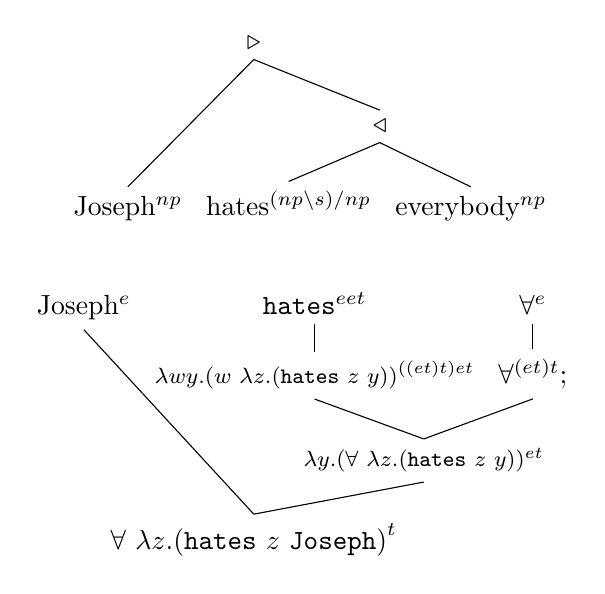
\begin{tikzpicture}
			\begin{scope}[frontier/.style={distance from root=60pt}]
			\Tree
			[.{$\triangleright$}
				\node(J){Joseph$^{np}$};
				[.{$\triangleleft$}
					\node(h){hates$^{(np\backslash s)/np}$};
					\node(e){everybody$^{np}$};
				]
			]
			\end{scope}
			\begin{scope}[yshift=-2.5in,frontier/.style={distance from root=85pt}, grow'=up]
			\Tree 
			[.{${\forall \ \lambda z.(\term{hates} \ z \ \term{Joseph})}^t$}
				{Joseph$^e$}
				[.{\footnotesize $\lambda y.(\forall \ \lambda z.(\term{hates} \ z \ y))^{et}$}
					[.{\footnotesize ${\lambda wy.(w \ \lambda z.(\term{hates} \ z \ y))}^{((et)t)et}$}
						\node(sh){$\term{hates}^{eet}$};
					]
					[.{$\forall^{(et)t}$};
						\node(set){$\forall^e$};
					]
				]
			]			
			\end{scope}		
		\end{tikzpicture}
	\]
\end{frame}

\begin{frame}{(2) Incremental CPS}
	\small
	\alert{Two translations} left-to-right $\barkr{(.)}$ and right-to-left incremental $\barkl{(.)}$
	
	For $A$ atomic, $\barkr{A} = \barkl{A} = (\trans{A} \li \bot)\li \bot$\footnote{$\bot$ the \textit{response} type, here $t$}
	\vfill

	For complex types, we have:
	\begin{itemize}
		\item Left-to-right $\barkr{(.)}$
		\begin{itemize}
			\item[] $\barkr{(N \triangleright M)} = 
				\lambda k.(\barkr{N} \ \lambda n.(\barkr{M} \ \lambda m.(k \ (m \ n))))$
			\item[] $\barkr{(M \triangleleft N)} =
				\lambda k.(\barkr{M} \ \lambda m.(\barkr{N} \ \lambda n.(k \ (m \ n))))$			
		\end{itemize}
		\item Right-to-left $\barkl{(.)}$
		\begin{itemize}
			\item[] $\barkl{(N \triangleright M)} = 
				\lambda k.(\barkl{M} \ \lambda m.(\barkl{N} \ \lambda n.(k \ (m \ n))))$
			\item[] $\barkl{(M \triangleleft N)} =
				\lambda k.(\barkl{N} \ \lambda n.(\barkl{M} \ \lambda m.(k \ (m \ n))))$
		\end{itemize}
	\end{itemize}
\end{frame}

\begin{frame}{(2) Incremental CPS: Example}
	\small
	\begin{center}
		\alert{Lexical Translation}\\
		
	\begin{tabularx}{0.7\textwidth}{lr}
	Source & Target\\
	\toprule
	 Joseph :: $np$ & $\lambda k.(k \ \term{Joseph})$ :: $(et)t$\\
	 hates :: $(np\backslash s)/np$ &$\lambda k.(k \ \term{hates})$ :: $((eet)t)t$ \\
	 everybody :: $np$ & $\forall$ :: $(et)t$
	\end{tabularx}
	\end{center}\vfill
	
	\pause
	\alert{Left-to-right translation}
	\begin{itemize}
		\item[] $\barkr{(N \triangleright M)} = 
			\lambda k.(\barkr{N} \ \lambda n.(\barkr{M} \ \lambda m.(k \ (m \ n))))$
		\item[] $\barkr{(M \triangleleft N)} =
			\lambda k.(\barkr{M} \ \lambda m.(\barkr{N} \ \lambda n.(k \ (m \ n))))$			
	\end{itemize}
	\vspace{-10pt}
	
	\pause
	{\footnotesize
	\begin{align*}
		\alt<7->{
		\hspace{-10pt}
			\barkr{(\text{J} \triangleright (\text{h} \triangleleft \text{e}))} 
			&= \lambda k_2.(\barkr{\text{Joseph}} \ \lambda n_2.(\barkr{(\text{hates} \triangleleft \text{everybody})} \ \lambda m_2.(k_2  \ (m_2 \ n_2)))))\\
			\visible<8->{&=  
			\lambda k_2.\left(
				% Joseph
				\textcolor{red}{
				\lambda k_3.\left(
					k_3 \ \term{Joseph}
				\right)
				}
				\ 
				\textcolor{gray}{
				\lambda n_2.\left(
					% hates everybody
					\barkr{(\text{hates} \triangleleft \text{everybody})}
					\ 
					\lambda m_2.\left(
						k_2 \ (m_2 \ n_2
					\right)
				\right)
				}
			\right)
			\\
			&\stackrel{\beta}{\rightsquigarrow}  
			\lambda k_2.\left(
				\textcolor{red}{
				\lambda n_2.\left(
					% hates everybody
					\barkr{(\text{hates} \triangleleft \text{everybody})}
					\ 
					\lambda m_2.\left(
						k_2 \ (m_2 \ n_2
					\right)
				\right)
				}
				\  
				\textcolor{gray}{
				\term{Joseph}
				}
			\right)
			\\
			& \stackrel{\beta}{\rightsquigarrow}
			\lambda k_2.\left(
				% hates everybody
				\barkr{(\text{hates} \triangleleft \text{everybody})}
				\ 
				\lambda m_2.\left(
					k_2 \ (m_2 \ \term{Joseph}
				\right)
			\right)
			\\
			& =\lambda k_2.\left(
				\textcolor{red}{
				% hates everybody
				\lambda k_1.\left(
					\forall  \
					\lambda m_1.\left(
						k_1 \ \left(
							\term{hates} \ m_1
						\right)
					\right)
				\right)
				}
				\ 
				\textcolor{gray}{
				\lambda m_2.\left(
					k_2 \ \left(m_2 \ \term{Joseph} \right)
				\right)
				}
			\right)
			\\
			& \stackrel{\beta}{\rightsquigarrow}\lambda k_2.\left(
				\forall  \
				\lambda m_1.\left(
					\textcolor{red}{
					\lambda m_2.\left(
						k_2 \ \left(m_2 \ \term{Joseph} \right)
					\right)
					}
					\
					\textcolor{gray}{\left(
						\term{hates} \ m_1
					\right)
					}
				\right)
			\right)
			\\
			& \stackrel{\beta}{\rightsquigarrow}\lambda k_2.\left(
				\forall  \
				\lambda m_1.\left(
					k_2 \ \left(
							\term{hates} \ m_1
						\
						\term{Joseph} 
					\right)
				\right)
			\right) \xrightarrow{\mathrm{eval}} \forall \lambda m_1.\left(\term{hates} \ m_1 \ \term{Joseph}\right)
			\\
			}
		}{
		\visible<3->{
		\barkr{(\text{h} \triangleleft \text{e})} &= 
		\lambda k_1.(\barkr{\text{hates}} \ \lambda n_1.(\barkr{\text{everybody}} \ \lambda m_1.(k_1 \ (m_1 \ n_1))))\\
		\visible<4->{
		& = \lambda k_1.(\textcolor{red}{\lambda k_0.(k_0 \ \term{hates})} \ \textcolor{gray}{\lambda n_1.(\forall \ \lambda m_1.(k_1 \ (m_1 \ n_1)))})\\
		\visible<5->{
		& \stackrel{\beta}{\rightsquigarrow} \lambda k_1.(\textcolor{red}{\lambda n_1.(\forall \ \lambda m_1.(k_1 \ (m_1 \ n_1)))} \ \textcolor{gray}{\term{hates}})\\
		\visible<6->{
		& \stackrel{\beta}{\rightsquigarrow} \lambda k_1.(\forall \ \lambda m_1.(k_1 \ (\term{hates} \ m_1))))
		}}}}}
	\end{align*}
	}
\end{frame}

\begin{frame}{(3) Plotkin's CPS Interpretation}
	\small
	New \textit{value} translation $\trans{.}$:\\
	\begin{center}
	$\trans{np} = e$, $\trans{s} = t$, $\trans{B/A} = \trans{A \backslash B} = \trans{A} \li (\trans{B} \li \bot) \li \bot$	
	\end{center}
	And \textit{computation} translation $\overline{A} = (\trans{A} \li \bot)\li \bot$ {\footnotesize(here: $\bot = t$)}.
	\vfill
	
	\begin{center}
	\alert{Lexical Translation}\\
	{\footnotesize
	\begin{tabularx}{0.99\textwidth}{@{}C@{}C@{}C@{}}
	Source & $\trans{.}$ & Target\\
	\toprule
	 Joseph :: $np$ & $e$ & $\lambda k.(k \ \term{Joseph}):: (et)t$\\
	 hates :: $(np\backslash s)/np$ &\alt<3->{$e\left(\left(e\left(tt\right)t\right) t\right)t$}{$?$} & \alt<4->{$? :: \left( \left( e\left(\left(e\left(tt\right)t\right) t\right)t \right)t\right)t$}{$?$} \\
	 everybody :: $np$ & $e$ & $\forall :: (et)t$
	\end{tabularx}
	}
	\end{center}\vfill
	
	\pause
	\alt<5->{
	\alert{Term Assignment}\\
	\begin{minipage}{0.55\textwidth}
	\footnotesize
	\[
	\underbrace{\left(
		\left( 
			\overbrace{e}^x 
			\underbrace{\left( 
				\left(
				\overbrace{e}^{y} 
				\overbrace{\left(tt\right)}^{\tau}t\right) t\right)
			}_{h}t 
		\right)t
	\right)}_{f}t
	\]	
	\end{minipage}%
	\begin{minipage}{0.5\textwidth}
	\footnotesize
	\[
		\visible<6->{\lambda f.\left(f \ \lambda xh.\left(h \ \lambda y\tau.\left(\tau \ \left(\term{hates}\ x\ y\right)\right)\right)\right)}
	\]
	\end{minipage}
	}{
	\begin{align*}
		\trans{np \backslash s} & = \trans{np} \li (\trans{s} \li \bot) \li \bot = e \li (t\li t) \li t = e\left(tt\right)t\\
		\visible<3->{\trans{(np \backslash s)/np} &= \trans{np} \li (\trans{np\backslash s} \li \bot) \li \bot = e\left(\left(e\left(tt\right)t\right) t\right)t\\}
		\visible<4->{\overline{(np\backslash s)/np} &= \left( \left( e\left(\left(e\left(tt\right)t\right) t\right)t \right)t\right)t}
	\end{align*}
	}
\end{frame}

\begin{frame}{(3) Plotkin's CPS Interpretation}
	\small
	\begin{center}
	\alert{Lexical Translation}\\
	{\footnotesize
	\begin{tabularx}{1.05\textwidth}{@{}lr@{}}
	Source &  Target\\
	\toprule
	 Joseph :: $np$ & $\lambda k.(k \ \term{Joseph}):: (et)t$\\
	 hates :: $(np\backslash s)/np$ & 
	 $\lambda f.(f \ \lambda xh.(h \ \lambda y\tau.(\tau \ (\term{hates}\ x\ y)))) :: ( ( e((e(tt)t) t)t )t)t$ \\
	 everybody :: $np$ & $\forall :: (et)t$
	\end{tabularx}
	}
	\end{center}\vfill
	
	\pause
	\alert{Term Translation}\\
	\begin{itemize}
		\item[] $\overline{M \triangleleft N} = \overline{N \triangleright M} = \lambda k.(\overline{M} \ \lambda m.(\overline{N} \ \lambda n.(m \ n \ k)))$
	\end{itemize}
	
	\footnotesize
	\begin{align*}
	\alt<6->{
	\hspace{-20pt}
		\overline{\text{J}\triangleright (\text{h} \triangleleft \text{e})} & = 
		\lambda k_2.\left(\overline{\text{h} \triangleleft \text{e}} \ \lambda m_2.\left(\textcolor{red}{\lambda k_3.\left(k_3 \ \term{Joseph}\right)} \ \textcolor{gray}{\lambda n_2.\left(m_2 \ n_2 \ k_2\right)}\right)\right) \\
		& \stackrel{\beta}{\rightsquigarrow} \lambda k_2.\left(\overline{\text{h} \triangleleft \text{e}} \ \lambda m_2.\left(\textcolor{red}{\lambda n_2.\left(m_2 \ n_2 \ k_2\right)} \ \textcolor{gray}{\term{Joseph}}\right)\right)\\
		& \stackrel{\beta}{\rightsquigarrow} \lambda k_2.\left(\overline{\text{h} \triangleleft \text{e}} \ \lambda m_2.\left(m_2 \ \term{Joseph} \ k_2\right)\right)\\
		& = 
		\lambda k_2.\left(
			\textcolor{red}{\lambda k.\left(
				\forall \
				\lambda n.\left(
					k \ \lambda y\tau.\left(
						\tau \ \left(
							\term{hates} \ n \ y
						\right)
					\right)				
				\right)
			\right)} \ 
			\textcolor{gray}{\lambda m_2.\left( m_2 \ \term{Joseph} \ k_2 \right)}
		\right)\\
		&= \lambda k_2.\left(
		\forall \
			\lambda n.\left(
				\textcolor{red}{\lambda m_2.\left( m_2 \ \term{Joseph} \ k_2 \right)} \
				 \textcolor{gray}{\lambda y\tau.\left(
					\tau \ \left(
						\term{hates} \ n \ y
					\right)
				\right)
				}	
			\right)
		\right)\\
		&= \lambda k_2.\left(
			\forall \
				\lambda n.\left(
					\textcolor{red}{\lambda y\tau.\left(
						\tau \ \left(
							\term{hates} \ n \ y
						\right)
					\right)
					}
					\ \textcolor{gray}{\term{Joseph} \ k_2}
				\right)
			\right)\\
		&= \lambda k_2.\left(
				\forall \
				\lambda n.\left(
					k_2 \ \left(\term{hates} \ n \ \term{Joseph}\right)
				\right)
			\right) \xrightarrow{eval} \forall \ \lambda n.\left( \term{hates} \ n \ \term{Joseph} \right)
	}{
		\overline{\text{h} \triangleleft \text{e}} &= 
		\lambda k.\left(
			\textcolor{red}{
			% hates
			\lambda f.\left(f \ \lambda xh.\left(h \ \lambda y\tau.\left(\tau \ \left(\term{hates}\ x\ y\right)\right)\right)\right)}
			\ \textcolor{gray}{\lambda m.\left(
			% everybody
				\forall
				\ \lambda n.\left(m \ n \ k\right)
			\right)
			}
		\right)\\
		& = \lambda k.\left(
			\textcolor{red}{
			\lambda m.\left(
				% everybody
				\forall
				\ \lambda n.\left(m \ n \ k\right)
			\right)}
			\
			\textcolor{gray}{\lambda xh.\left(h \ \lambda y\tau.\left(\tau \ \left(\term{hates}\ x\ y\right)\right)\right)}
		\right) \\
		& = \lambda k.\left(
				% everybody
				\forall
				\ \lambda n.\left(
					\textcolor{red}{\lambda xh.\left(h \ \lambda y\tau.\left(\tau \ \left(\term{hates}\ x\ y\right)\right)\right)}
				\ \textcolor{gray}{n \ k}\right)
			\right) \\
		&= \lambda k.\left(
				\forall \
				\lambda n.\left(
					k \ \lambda y\tau.\left(
						\tau \ \left(
							\term{hates} \ n \ y
						\right)
					\right)				
				\right)
			\right)
	}
	\end{align*}
\end{frame}

\end{document}